% ----------------------------------------------------------------------------
% Section 12.10 --- Structural Interpretation: Projective Thermodynamics
% From former §15.10, condensed
% ----------------------------------------------------------------------------
\subsection{Structural Interpretation: Projective Thermodynamics}
\label{subsec:structural-interpretation-projective-thermodynamics}

Physical observables arise through a generically non-injective projection
$\Pi : \Omega \rightarrow O$.
In saturation regimes, the resulting loss of distinguishability induces a
structural entropy:
\begin{equation}
  S_{\Pi} = -\sum_{o \in O}
    \mu(\Pi^{-1}(o)) \log \mu(\Pi^{-1}(o)),
\end{equation}
which is an objective property of the projection.

\begin{figure}[t]
  \centering
  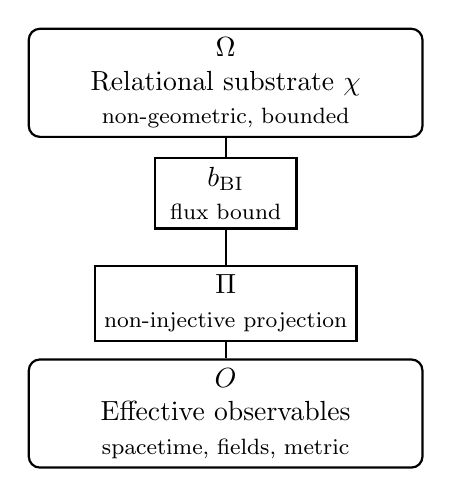
\begin{tikzpicture}[
    node distance=1.4cm,
    every node/.style={align=center},
    box/.style={draw, rounded corners, thick,
      minimum width=5cm, minimum height=1cm},
    narrow/.style={draw, thick,
      minimum width=1.8cm, minimum height=0.8cm}
  ]
    \node[box] (omega)
      {$\Omega$\\Relational substrate $\chi$\\
       {\footnotesize non-geometric, bounded}};
    \node[narrow, below of=omega] (bi)
      {$b_{\mathrm{BI}}$\\
       {\footnotesize flux bound}};
    \node[narrow, below of=bi] (pi)
      {$\Pi$\\
       {\footnotesize non-injective projection}};
    \node[box, below of=pi] (obs)
      {$O$\\Effective observables\\
       {\footnotesize spacetime, fields, metric}};
    \draw[thick] (omega) -- (bi);
    \draw[thick] (bi) -- (pi);
    \draw[thick] (pi) -- (obs);
  \end{tikzpicture}
  \caption{Projective regimes in Cosmochrony.
    The substrate~$\Omega$ undergoes bounded relaxation
    ($b_{\mathrm{BI}}$).
    Observables arise through non-injective projection~$\Pi$.}
  \label{fig:projective-hourglass}
\end{figure}

Effective parameters such as temperature or metric curvature emerge as
Lagrange multipliers absorbing unresolved relational complexity.
High effective temperatures or anomalous geometric features reflect the
compression of a bounded relational flux into a reduced observable
description, not excess local energy density.
The bounded character of substratic relaxation ensures that
projection-induced quantities remain finite, rendering the framework
predictive despite the non-injective nature of the projection.
